\begin{abstract}
Cumacea (crustaceans: Peracarida) are vital indicators of benthic health in marine ecosystems. This study investigated the influence of ecological and geographic parameters on their genetic variability in the Northern North Atlantic, focusing on Icelandic waters. We analyzed mitochondrial sequences of the 16S rRNA gene from 62 cumaceans specimens. Using the \textit{aPhyloGeo} software, we correlated these sequences with relevant factors such as latitude (decimal degree) at the start of sampling, wind speed (m/s) at the start of sampling, O\textsubscript{2} concentration (mg/L), and depth (m) at the beginning of sampling.

Our analyses revealed variability in geographic and environmental parameters, reflecting diverse ecological requirements and benthic habitats. The most common cumacean families, Diastylidae and Leuconidae, suggest adaptations to various marine environments. Phylogeographic analysis showed that specific genetic sequences were correlated with wind speed (m/s) at the start of sampling and O\textsubscript{2} concentration (mg/L). This indicates potential local adaptation to these fluctuating conditions.

These results reinforce the importance of further research into the relationship between cumacean genetics and environmental attributes. Understanding these relationships is crucial for elucidating the evolutionary dynamics in marine ecosystems. This study sheds essential light on invertebrate acclimatization to climate change and deep-sea habitat management. The results can contribute to the evolution of more efficient conservation strategies and inform policies that protect vulnerable marine ecosystems. 

The \textit{aPhyloGeo} Python package is freely and publicly available on \href{https://github.com/tahiri-lab/aPhyloGeo}{GitHub} and \href{https://pypi.org/project/aphylogeo/}{PyPi}, providing an invaluable tool for future research.
\end{abstract}

\section{Introduction}\label{introduction}
The North Atlantic and Subarctic regions, particularly the Icelandic waters, are of ecological interest due to their diverse water masses and unique oceanographic features \citep{schnurr_composition_2014, meisner_benthic_2014, uhlir_adding_2021}. These areas form vital {benthic habitats}\footnote{These are areas on the bottom of the oceans or lakes, including sediments and organisms that live in them.} \citep{levin2009ecological} and enhance our understanding of deep-sea ecosystems and biodiversity patterns \citep{rogers2007corals, danovaro2008exponential, uhlir_adding_2021}. The IceAGE project and its predecessors, BIOFAR and BIOICE, provide invaluable data for studying the impacts of climate change and seabed mining, especially in the Greenland, Iceland, and Norwegian (GIN) seas \citep{meisner_prefacebiodiversity_2018}. 

Cumacea, a crustacean taxon within Peracarida, provide major indicators of marine ecosystem health due to their sensitivity to environmental fluctuations \citep{stransky_diversity_2010} and their contribution to benthic foods webs \citep{rehm2009cumacea}. Despite their ecological importance, deep-sea benthic invertebrates’ evolutionary history and dynamics remain uncharted, notably in the North Atlantic. Understanding these deep-sea organisms' genetic distribution and demography is central for predicting their response to climate change \citep{jennings_phylogeographic_2014}. 

Considering the current climate emergency, this study aims to analyze the influence of geographical, environmental, and climatic parameters on the genetics of cumacean in the Nothern North Atlantic. Specifically, we will examine whether there is a correlation between the 16S rRNA mitochondrial gene region of cumacean species sampled and their habitat characteristics. If so, we will determine which attributes correlate best with a specific genetic sequence (i.e., window) and identify the potential associated protein. Our approach includes confirming different {phylogeographic models}\footnote{Phylogeographic models are computational tools that analyze relationships between the genetic structures of populations and their geographic distributions. In our case, by incorporating geographic, environmental, and climatic properties, we can interpret their impact on the genetic distribution of cumacean species.} and updating a Python package (currently in beta), \textit{aPhyloGeo}, to simplify these analyses.

This paper is structured as follows: Section \autoref{related-works} reviews pertinent studies on the biodiversity and biogeography of deep-sea benthic invertebrates; Section \autoref{contribution} summarizes the aims and contributions of this study, highlighting aspects relating to the conservation and acclimatization of marine invertebrates to climate change; Section \autoref{materials-methods} details the data collection, sampling procedures, and genetic analyses; Section \autoref{metrics} describes the metrics used for evaluating phylogeographic models; Section \autoref{results} presents the findings; and Section \autoref{conclusion}  discusses their implications for future research and conservation efforts.

\section{Related Works}\label{related-works}
Assessing and quantifying the biodiversity of deep-sea benthic invertebrates has become increasingly crucial since it was discovered that their richness may be underestimated \citep{grassle1992deep}. Subsequent research has highlighted the need for large-scale distribution models to interpret the diversity of these organisms across their ecological and evolutionary contexts \citep{rex1997large}. That is why recent efforts have focused on mapping, managing, and studying the seabed. Advanced technologies such as acoustic detection are improving our knowledge of benthic ecosystem complexity \citep{brown2011benthic}. Integrating genetic and habitat characteristics gives a deeper understanding of how ecological and geographic factors influence the genetic differences, distribution, biodiversity, and resilience of deep-sea benthic organisms \citep{vrijenhoek2009cryptic}.

However, the relationship between genetics and the environment is complex, involving gene-environment interactions and natural selection factors, which makes it difficult to identify clear causal relationships \citep{balkenhol_identifying_2009}. In addition, the distinction between the direct and indirect effects of the environment on genetics poses other challenges \citep{manel_perspectives_2010, balkenhol_landscape_2019}. The restrictions of available methods for measuring genetic and ecological attributes, combined with logistical constraints, often limit the scope of such studies \citep{manel_perspectives_2010, shafer_widespread_2013}. This complexity may explain why the environment and genetics of cumaceans have been less studied, even though they are essential for interpreting how these deep-sea invertebrates adapt to fluctuating environmental conditions.

\section{Our Contribution}\label{contribution}
Our study focuses on the genetic variation of the 16S rRNA mitochondrial gene in cumacean populations in the face of environmental fluctuations, which has been little explored in previous studies \citep{grassle1992deep, rex2000latitudinal}. We aim to refine the natural selection hypothesis by identifying the genetic region with the highest mutation rate based on the fact that individuals best adapted to their environment are likely to survive and evolve. We then analyze its correlation with geographical and ecological distribution patterns and determine the protein potentially associated with this region. This method represents a major advance over previous research, which often fails to integrate genetic and environmental data in the context of deep-sea invertebrates \citep{etter1990population, vrijenhoek2009cryptic}.

Using robust analytical methods such as dissimilarity calculations and phylogenetic reconstructions, we provide new insights into the genetic adaptation of marine cumaceans. Unlike previous studies, which have encountered difficulties establishing a link between genetics and the environment \citep{manel2003landscape, balkenhol2009statistical}, our results provide a better understanding of evolutionary dynamics in aquatic ecosystems.

Furthermore, our genetic and environmental data highlights critical habitats of high conservation interest, which can be considered for establishing marine protected areas \citep{levin2009ecological}. These results are essential for developing informed conservation strategies in the context of climate change. Finally, our study paves the way for further research on other invertebrate species across different geographical regions. By extending this research to diverse environments and taxonomic groups, scientists will gain a more complete understanding of the adaptation and resilience of marine invertebrates to changing conditions. This work contributes essential insights to the field and supports the development of informed conservation strategies.

\section{Materials and Methods}\label{materials-methods}
This section describes our data and introduces the main stages of data pre-processing and the \textit{aPhyloGeo} software. A flow chart, constructed with the diagram software draw.io, summarizes this section (see Figure \ref{fig:fig1} below).

\begin{figure}[htbp]
    \centering
    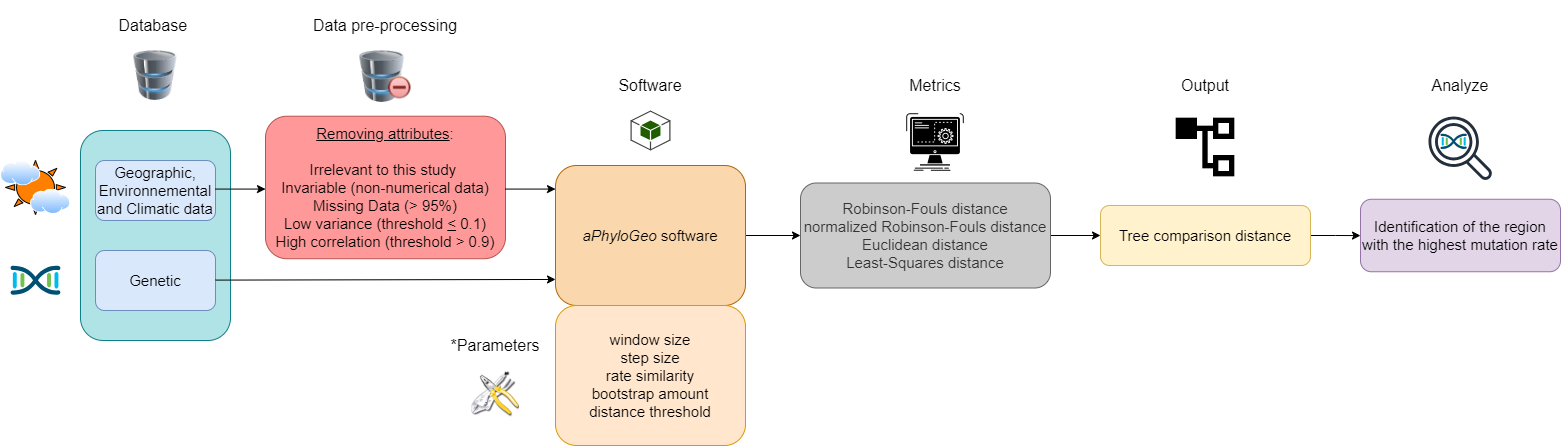
\includegraphics[width=0.7\textwidth]{diagram.drawio.png}
    \caption{Flow chart summarizing the Materials and Methods section workflow. Six different colors highlight the blocks. The first block (blue) represents our database. The second block (red) is data pre-processing, where we remove attributes. The third and fourth blocks (orange) implement the \textit{aPhyloGeo} software and its parameters for our phylogeographic analyses. The fifth block (grey) calculates phylogenetic tree comparison distances. The sixth block (yellow) compares the distances between the phylogenetic trees produced. The seventh block (purple) identifies regions with high mutation rates based on the results of the tree comparisons. *See YAML file on \href{https://github.com/tahiri-lab/aPhyloGeo}{GitHub}. \label{fig:fig1}}
\end{figure}

\subsection{Description of the data}
The study area was located in a northern region of the North Atlantic, including the Icelandic Sea, the Denmark Strait, and the Norwegian Sea. The specimens examined were collected as part of the IceAGE project (Icelandic marine Animals: Genetic and Ecology; Cruise ship M85/3 in 2011), which studied the deep continental slopes and abyssal waters around Iceland \citep{meisner_prefacebiodiversity_2018}. The sampling period for the included specimens was from August 30 to September 22, 2011, and they were collected at depths ranging from 316 to 2568 m. Information on the sampling plan, sample processing, DNA extraction steps, PCR amplification, sequencing, and extracted and aligned DNA sequences is available in the \citep{uhlir_adding_2021} article.

\subsection{Data pre-processing}
We used data from the IceAGE project and related data from the bold system's database, both accessible \emph{via} the \citep{uhlir_adding_2021}. Given these databases' enormous breadth of attributes, we selectively reduced the number of attributes and samples. Particularly, we have omitted attributes that were not directly relevant to the analysis of correlations between cumacean genetics and habitat attributes, had little to no variability (non-numerical data), and had a large number of missing data (>95\%). In the IceAGE dataset, we considered 62 specimens out of the 495 available, as only these had their mitochondrial DNA sequence of the 16S rRNA gene. 

Next, we calculated the variance using the var() function in RStudio Desktop 4.3.2 for each of the selected numerical attributes to eliminate those with zero or low variance (threshold ≤ 0.1). The formula (equation \ref{variance}) and code (\autoref{lst:variance}) used to calculate the variance of our final attributes, available on \href{https://github.com/tahiri-lab/Cumacea_aPhyloGeo}{GitHub}, are provided below:

\begin{equation}\label{variance}
    S^2 = \frac{\sum_{i=1}^{n} (x_i - \bar{x})^2}{n-1}
\end{equation}

where $S^2$ is the variance of the attribute, $x_i$ represents each attribute value, $\bar{x}$ is the average of the values for this attribute, and $n$ is the number of values for this attribute in the dataset.

%\autoref{lst:variance}.
\begin{lstlisting}[label=lst:variance,language=RStudio,caption=RStudio script to calculate the variance of each numerical attributes in our final dataset]
# Import data
Data <- read.csv(file = "Final_Data_Article.csv", header = TRUE, sep = ";")

# Calculate the variance of numerical attributes only from the dataset
variances <- sapply(Data, function(x) {
  if (is.numeric(x)) {
    var(x, na.rm = TRUE)
  } else {
    NA
  }
})

# Display variances
print(variances)
\end{lstlisting}

Only water salinity has been removed from the previously selected numerical attributes ($S^2 = 0.02146629$). We then eliminated attributes that showed strong correlations with each other (threshold > 0.90) using the cor() function in RStudio Desktop 4.3.2 to avoid repetition between attributes and ensure that each was unique and relevant. Since we have three missing data for the attribute of water O\textsubscript{2} concentration, we have used the "pairwise.complete.obs method". This method calculates the Pearson correlation matrix using all accessible pairs of observations, even if some data are missing. The formula (equation \ref{pearson}) and code (\autoref{lst:pearson}) used to calculate the Pearson correlation coefficient of our final attributes are shown below:

\begin{equation}\label{pearson}
    r = \frac{\sum_{i=1}^{n} (x_i - \bar{x})(y_i - \bar{y})}{\sqrt{\sum_{i=1}^{n} (x_i - \bar{x})^2 (y_i - \bar{y})^2}}
\end{equation}

where $r$ is the Pearson correlation coefficient between two attributes, $x_i$ are the values of an attribute, $y_i$ are the values of another attribute, $\bar{x}$ and $\bar{y}$ are respectively the averages of the two attributes, and $n$ is the sample size of the two attributes.

%\autoref{lst:pearson}.
\begin{lstlisting}[label=lst:pearson,language=RStudio,caption=RStudio script to calculate the Pearson correlation coefficient between all the numerical attributes in our final dataset]
# Import data
Data <- read.csv(file = "Final_Data_Article.csv", header = TRUE, sep = ";")

# Select numeric columns only from the dataset
numeric_Data <- Data[sapply(Data, is.numeric)]

# Calculate Pearson correlation matrix
correlation_matrix <- cor(numeric_Data, use = "pairwise.complete.obs")

# Display correlation matrix
print(correlation_matrix)
\end{lstlisting}

This selection of attributes and data resulted in a table containing 62 rows ($n=62$) and 17 columns (number of attributes). 

\subsection{Selected attributes in the IceAGE database}

\subsubsection{Geographic attributes} 

\begin{itemize}
\item The latitude (Figure \ref{fig:fig2}a) and longitude (Figure \ref{fig:fig2}b) at the start of sampling, both in decimal degrees (DD).
\item The sectors across the seas around Iceland: the Denmark Strait ($n=28$), the Iceland Basin ($n=15$), the Irminger Basin ($n=12$), the Norwegian Sea ($n=4$), and the Norwegian Basin ($n=3$). 
\end{itemize}

\subsubsection{Environmental attributes} 
\begin{itemize}
\item Depth (m) at the start of sampling (Figure \ref{fig:fig2}c), as well as temperature ($^\circ$C) (Figure \ref{fig:fig2}e) and O\textsubscript{2} concentration (mg/L) (Figure \ref{fig:fig2}f) of the water as a function of the depth at which specimens were sampled. 
\item The sedimentary characteristics of the sampling sites, which influence the distribution of Cumacea \citep{uhlir_adding_2021}. In this study, they fall into six categories: mud ($n=30$), sandy mud ($n=15$), sand ($n=9$), forams ($n=3$), muddy sand ($n=3$), and gravel ($n=2$).
\end{itemize}

\subsubsection{Climatic attributes} 
Wind speed (m/s) (see Figure \ref{fig:fig2}d) and wind direction at the start and end of sampling were also included, given the contribution of wind to the restructuring of the benthic ecosystem through water transport \citep{waga_recent_2020,saeedi_environmental_2022}. The wind direction at the start of sampling comprises six orientations: South-West ($n=22$), South ($n=15$), North-East ($n=9$), South-South-East ($n=9$), North-West ($n=5$), and East ($n=2$); while that at the end of sampling is composed of seven orientations: South ($n=15$), South-West ($n=15$), North-East ($n=9$), West-South-West ($n=7$), South-East ($n=6$), North-North-West ($n=5$), South-South-East ($n=3$), and East ($n=2$). 

\subsection{Selected attributes in the bold system's database}
\subsubsection{Taxomic attributes} 
The family, genus, and scientific name of the cumacean sampled have been integrated into our data. These comprise seven families: Diastylidae ($n=21$), Lampropidae ($n=13$), Leuconidae ($n=12$), Astacidae ($n=7$), Bodotriidae ($n=4$), Ceratocumatidae ($n=3$), and Pseudocumatidae ($n=2$). A total of 21 cumacean species were found in our sample (see Figure \ref{fig:fig3}).

We also included the sample identity (id) of each cumacean sampled. Some specimens were identified only to genus (one specimen) or family (five specimens) in our sample.

\subsection{Selected attributes from article \cite{uhlir_adding_2021}} 
\subsubsection{Other environmental attributes} 
The habitat and water mass of the sampling points were the only attributes taken directly from Table 1 of \citep{uhlir_adding_2021}. Thus, the water mass definitions described by \citep{hansen_north_2000, brix2010distribution, ostmann_marine_2014} were used as a reference for the GIN seas around Iceland: Arctic Polar Water (APW, $n=15$), Iceland Sea Overflow Water (ISOW, $n=15$), North Atlantic Water (NAW, $n=9$), Arctic Polar Water/Norwegian Sea Arctic Intermediate Water (APW/NSAIW, $n=7$), warm Norwegian Sea Deep Water (NSDWw, $n=8$), Labrador Sea Water (LSW, $n=3$), cold Norwegian Sea Deep Water (NSDWc, $n=3$), and Norwegian Sea Arctic Intermediate Water (NSAIW, $n=2$) (see Figure \ref{fig:fig4}). In terms of habitat, we considered the three categories used in \citep{uhlir_adding_2021}: deep sea ($n=38$), shelf ($n=15$), and slope ($n=9$) (see Figure \ref{fig:fig5}).

To better interpret benthic species' relationship and evolutionary responses, genetic data are required \citep{wilson_speciation_1987, uhlir_adding_2021}. Thus, the aligned DNA sequence of the 16S rRNA mitochondrial gene region from each of the samples was included in our analyses. This region is standard in phylogeny and phylogeography studies \citep{hugenholtz1998impact} and sufficiently conserved over time to guarantee exact alignments between different species or populations \citep{saccone1999evolutionary}. We examined 62 of the 306 aligned DNA sequences used for phylogeographic analyses by \citep{uhlir_adding_2021}. As some specimens in our sample have their DNA sequence duplicated, or even quadruplicated with a difference of one or two nucleotides, we took into account the longest-aligned DNA sequence of each specimen.

\subsection{{\textit{aPhyloGeo} software}\label{aPhyloGeo-software}}
We used the cross-platform Python software \textit{aPhyloGeo} for our phylogeographic analyses, designed to analyze phylogenetic trees using ecological and geographic parameters \citep{koshkarov_phylogeography_2022}. Developed by My-Linh Luu, Georges Marceau, David Beauchemin, and Nadia Tahiri, \textit{aPhyloGeo} offers tools for the study of correlations between species genetics and habitat characteristics, helping to understand the evolution of species under different environmental conditions \citep{koshkarov_phylogeography_2022}. 

We selected this software for our analysis because, to our knowledge, it is the first phylogeographic tool capable of correlating species genetics with climatic, environmental, and geographical attributes - precisely the objective of our study \citep{koshkarov_phylogeography_2022}. \textit{aPhyloGeo} offers several  key functionalities:

\begin{enumerate}[label=\arabic*.]
\item Phylogeographic tree evaluation: The software elucidates evolutionary relationships between species based on their genetic sequences, which is essential for interpreting phylogeographical patterns \citep{koshkarov_phylogeography_2022}.
\item Ecological and geographic correlation analysis: It enables correlations between genetic sequences and the mentioned parameters to be tested and visualized. These correlations are crucial for identifying their influence on genetic fluctuations \citep{koshkarov_phylogeography_2022}.
\item Investigation of genetic diversity: \textit{aPhyloGeo} measures genetic heterogeneity based on geographic variation, enabling the recognition of potential local adaptations and evolutionary processes \citep{manel_perspectives_2010}.
\end{enumerate}

The \textit{aPhyloGeo} Python package is freely and publicly available on \href{https://github.com/tahiri-lab/aPhyloGeo}{GitHub}, and is also available on \href{https://pypi.org/project/aphylogeo/}{PyPi}, to facilitate complex phylogeographic analyses. The software process has three main stages (see \autoref{lst:main}).

%\autoref{lst:main}.
\begin{lstlisting}[label=lst:main,language=Python,caption=Main script for tutorial using the aPhyloGeo package.]
if __name__ == "__main__":

    # Load parameters
    Params.load_from_file()

    # Load the sequence file
    sequence_file = utils.load_sequence_file(Params.reference_gene_filepath)

    # Create an AlignSequences object
    align_sequence = AlignSequences(sequence_file)

    # Load attribute data 
    attribute_data = pd.read_csv(Params.file_name)

    # Perform the alignment of sequences
    alignments = align_sequence.align()

    # Generate phylogenetic trees
    genetic_trees = utils.genetic_pipeline(alignments.msa)
    
    # Create a GeneticTrees object
    trees = GeneticTrees(trees_dict=genetic_trees, format="newick")
   
    # Generate attribute trees
    attribute_trees = utils.attribute_pipeline(attribute_data)
    
    # Filter the results
    utils.filter_results(attribute_trees, genetic_trees, attribute_data)
\end{lstlisting}

\begin{enumerate}
\item \textbf{The first step} is to collect cumacean DNA sequences of sufficient quality for the needs of our results \citep{koshkarov_phylogeography_2022}. 62 cumaceans samples were selected to represent 62 16S rRNA mitochondrial gene sequences. We then included two climatic factors, namely wind speed (m/s) at the start and end of the sampling. We also included three environmental factors, such as sampling depth (m) at the start of sampling, temperature ($^\circ$C), and water O\textsubscript{2} concentration (mg/L). Finally, we integrated two geographical parameters, latitude (DD) and longitude (DD) at the start of sampling.

\item \textbf{In the second step}, trees were generated with environmental, geographical, climatic, and genetic data. Concerning geographical parameters, we calculated the dissimilarity between each data pair from different geographical conditions, producing a symmetrical square matrix. The {neighbor-joining algorithm}\footnote{It is a method used to construct phylogenetic trees using distance matrices.} was used to design the geographic tree from this matrix. The same approach was applied to environmental, climatic, and genetic data. An {iterative phylogenetic reconstruction method}\footnote{This method makes it possible to build phylogenetic trees by progressively reforming them as new data or sequences are added.} was used to construct phylogenetic trees based on 62 16S rRNA mitochondrial sequences, taking into account only data located within an interval that moves along the alignment. This displacement can vary according to the steps and the size of the window defined by the user (their length is determined by the number of base pairs (bp)) \citep{koshkarov_phylogeography_2022}.

\item \textbf{In the third step}, the phylogenetic trees constructed in each sliding window are compared with environmental, climatic, and geographic parameters using Robinson-Foulds Distance \citep{robinson_comparison_1981, koshkarov_phylogeography_2022}, normalized Robinson-Foulds Distance, Euclidean Distance, and Least-Squares Distance. These contribute to the understanding of similarities and dissimilarities between cumacean genetic sequences. The approach also takes bootstrapping into account. A sliding window allows detailed identification of regions with high genetic mutation rates.
\end{enumerate}

\subsection{Figure construction}
Figure \ref{fig:fig2}, Figure \ref{fig:fig3}, Figure \ref{fig:fig6} and Figure \ref{fig:fig7} were made with Python 3.11, while Figure \ref{fig:fig4} and Figure \ref{fig:fig5} were made with RStudio Desktop 4.3.2.

\section{Metrics}\label{metrics}
The following section presents a more concise version of the formulas mentioned in the third step of the \autoref{aPhyloGeo-software} section:

\subsection{Robinson-Foulds Distance}\label{RF}

The Robinson-Foulds Distance (RFD) quantifies dissimilarity between phylogenetic trees by counting the number of clades  (i.e., groups of species with a common origin) present in one tree but absent in the other. This measure can be used to assess topological differences between trees (see Equation \eqref{eq:rf} and \autoref{lst:robinsonFoulds}). 

In this context, we compare phylogenetic trees constructed from various habitat attributes (see the list in the first step of \autoref{aPhyloGeo-software}). For example, consider one tree based on habitat attribute A and the other trees based on the other habitat attributes (B, C, D, E, ...). The RFD measures the number of clades that differ between the initial tree (constructed using the A attribute) and each of the other trees, by calculating the level of topological dissimilarity between the trees. A high distance implies that the habitat attribute has a particular impact on the phylogenetic relationships of cumacean species compared to other attributes.

\begin{equation}\label{eq:rf}
    \text{RF}(T_1, T_2) = | \Sigma(T_1) \Delta \Sigma(T_2) |
\end{equation}

where $\Sigma(T_1)$ and $\Sigma(T_2)$ are the sets of splits in trees $T_1$ and $T_2$.

%\autoref{lst:robinsonFoulds}.
\begin{lstlisting}[label=lst:robinsonFoulds,language=Python,caption=Python script for calculating the RFD using the ete3 package in the aPhyloGeo package.]
import ete3

def robinson_foulds(tree1, tree2):
    rf = 0
    tree1_newick = ete3.Tree(tree1.format("newick"), format=1)
    tree2_newick = ete3.Tree(tree2.format("newick"), format=1)

    rf, rf_max, common_leaves = tree1_newick.robinson_foulds(tree2_newick, 
                                                             unrooted_trees=True)
    if len(common_leaves) == 0:
        rf = 0

    return rf, rf / rf_max
\end{lstlisting}

\subsection{Normalized Robinson-Foulds Distance}\label{RFnorm}

The normalized Robinson-Foulds Distance (nRFD) scales the RFD to account for the size variations in the trees (number of clades), allowing a more equitable comparison. It scales the distance to a range between 0 and 1. In our context, the distance has been normalized by $2n-6$, where $n$ represents the number of taxa. (see Equation \eqref{eq:rf_norm} and \autoref{lst:euclideanDist}).

For example, if the size of tree A differs due to missing data, this normalized metric allows us to compare its dissimilarity with that of other trees (B, C, D, ...) in a fairer way. In this case, it reveals the relative influence of habitat parameter A on cumacean phylogenetic relationships, independent of tree size.

\begin{equation}\label{eq:rf_norm}
    \text{RF}_{\text{norm}}(T_1, T_2) = \frac{| \Sigma(T_1) \Delta \Sigma(T_2) |}{| \Sigma(T_1) | + | \Sigma(T_2) |}
\end{equation}

\subsection{Euclidean Distance}\label{euclidean}

Euclidean Distance (ED) measures the distance between two points in a multi-dimensional space. In our study, it is used to compare vectors of habitat attributes between species (see Equation \eqref{eq:euclidean} and \autoref{lst:euclideanDist}).

By converting habitat attribute values into vectors, we measure the ED between vectors to quantify the dissimilarity between them of different cumacean species. This distance allows us to interpret how these differences influence their evolutionary relationships. For instance, species with similar habitat attribute vectors (low ED) may share closer evolutionary relationships. In contrast, those with a large difference in habitat vectors (high ED) may reveal evolutionary divergences.

For vectors $\mathbf{p} = (p_1, \ldots, p_n)$ and $\mathbf{q} = (q_1, \ldots, q_n)$, the ED between these vectors is calculated as:

\begin{equation}\label{eq:euclidean}
    d_{\text{Euclidean}}(\mathbf{p}, \mathbf{q}) = \sqrt{\sum_{i=1}^{n} (p_i - q_i)^2}
\end{equation}

where $p_i$ and $q_i$ are the components of the vectors.

%\autoref{lst:euclideanDist}.
\begin{lstlisting}[label=lst:euclideanDist,language=Python,caption=Python script for calculating the ED using the ete3 package in the aPhyloGeo package]
import dendropy

def euclidean_dist(tree1, tree2):
    tns = dendropy.TaxonNamespace()

    tree1_tc = dendropy.Tree.get(
        data=tree1.format("newick"), 
        schema="newick", 
        taxon_namespace=tns
    )
    
    tree2_tc = dendropy.Tree.get(
        data=tree2.format("newick"), 
        schema="newick", 
        taxon_namespace=tns
    )

    tree1_tc.encode_bipartitions()
    tree2_tc.encode_bipartitions()

    ed = dendropy.calculate.treecompare.euclidean_distance(tree1_tc, tree2_tc)

    return ed
\end{lstlisting}

\subsection{Least-Squares Distance}\label{LS}

The Least squares Distance (LSD) measures the differences between observed and the estimated values by summing the squares of these differences. In the context of phylogeographic trees, it quantifies the overall topological dissimilarity, considering the positions of nodes and branches (see Equation \eqref{eq:ls} and \autoref{lst:LeastSquare}).

This metric allows us to understand how these different habitat attributes influence the topological structure of phylogenetic trees. For example, by comparing a tree constructed from the habitat attribute A with trees built from other attributes, the LSD reveals the impact, high or low, of attribute A on changes in branch position and length.

\begin{equation}\label{eq:ls}
    d_{\text{LS}} = \sum_{i=1}^{n} (y_i - \hat{y}_i)^2
\end{equation}

where $y_i$ and $\hat{y}_i$ are the observed and estimated values, respectively.

%\autoref{lst:LeastSquare}.
\begin{lstlisting}[label=lst:LeastSquare, language=Python, caption=Python script for calculating the LSD using the ete3 package in the aPhyloGeo package]
def least_square(tree1, tree2):
    ls = 0.0
    leaves = tree1.get_terminals()

    leaves_name = [leaf.name for leaf in leaves]
    
    for i in leaves_name:
        leaves_name.pop(0)
        for j in leaves_name:
            d1 = tree1.distance(tree1.find_any(i), tree1.find_any(j))
            d2 = tree2.distance(tree2.find_any(i), tree2.find_any(j))
            ls += abs(d1 - d2)
    
    return ls
\end{lstlisting}

Our phylogeographic study used these four metrics to quantify topological differences between phylogenetic trees and assess dissimilarities between genetic sequences and environmental, geographical, and climatic features. The result is a comprehensive analysis of the evolutionary dynamics of cumacean populations in different contexts.

\section{Results}\label{results}
To understand the correlation between cumacean genetics and habitat, we parameterized the software \textit{aPhyloGeo} as follows: pairwiseAligner, Hamming distance, Wider Fit by elongating with Gap (starAlignment), windows size: 1 nucleotide (nt) and window step: 10 nt. The results of the metrics used were obtained using the functions leastSquare(tree1, tree2), robinsonFoulds(tree1, tree2), euclideanDist(tree1, tree2) from the \textit{aPhyloGeo} software and were organized by the main function (see \autoref{lst:main}). A more in-depth analysis of the results presented below is available on \href{https://github.com/tahiri-lab/Cumacea_aPhyloGeo}{GitHub} in the supplementary file.

The violon diagrams shown in Figure \ref{fig:fig2} are used to display summary statistics similar to box plots, showing medians (white dots), interquartile ranges (thickened black bars), and the rest of the distributions (thin black lines), except the "extreme" points. Wider areas indicate a greater probability of the variables taking a given value. They summarize the distribution of geographical (latitude and longitude at the start of sampling (DD)), climatic (wind speed (m/s) at the start of sampling), and environmental (depth (m) at the beginning of sampling, water temperature ($^\circ$C), and O\textsubscript{2} concentration (mg/L)) data. These diagrams are essential for understanding habitat conditions and highlighting unique habitats that can potentially influence cumacean genetic adaptability. 

\begin{figure}[htbp]
    \centering
    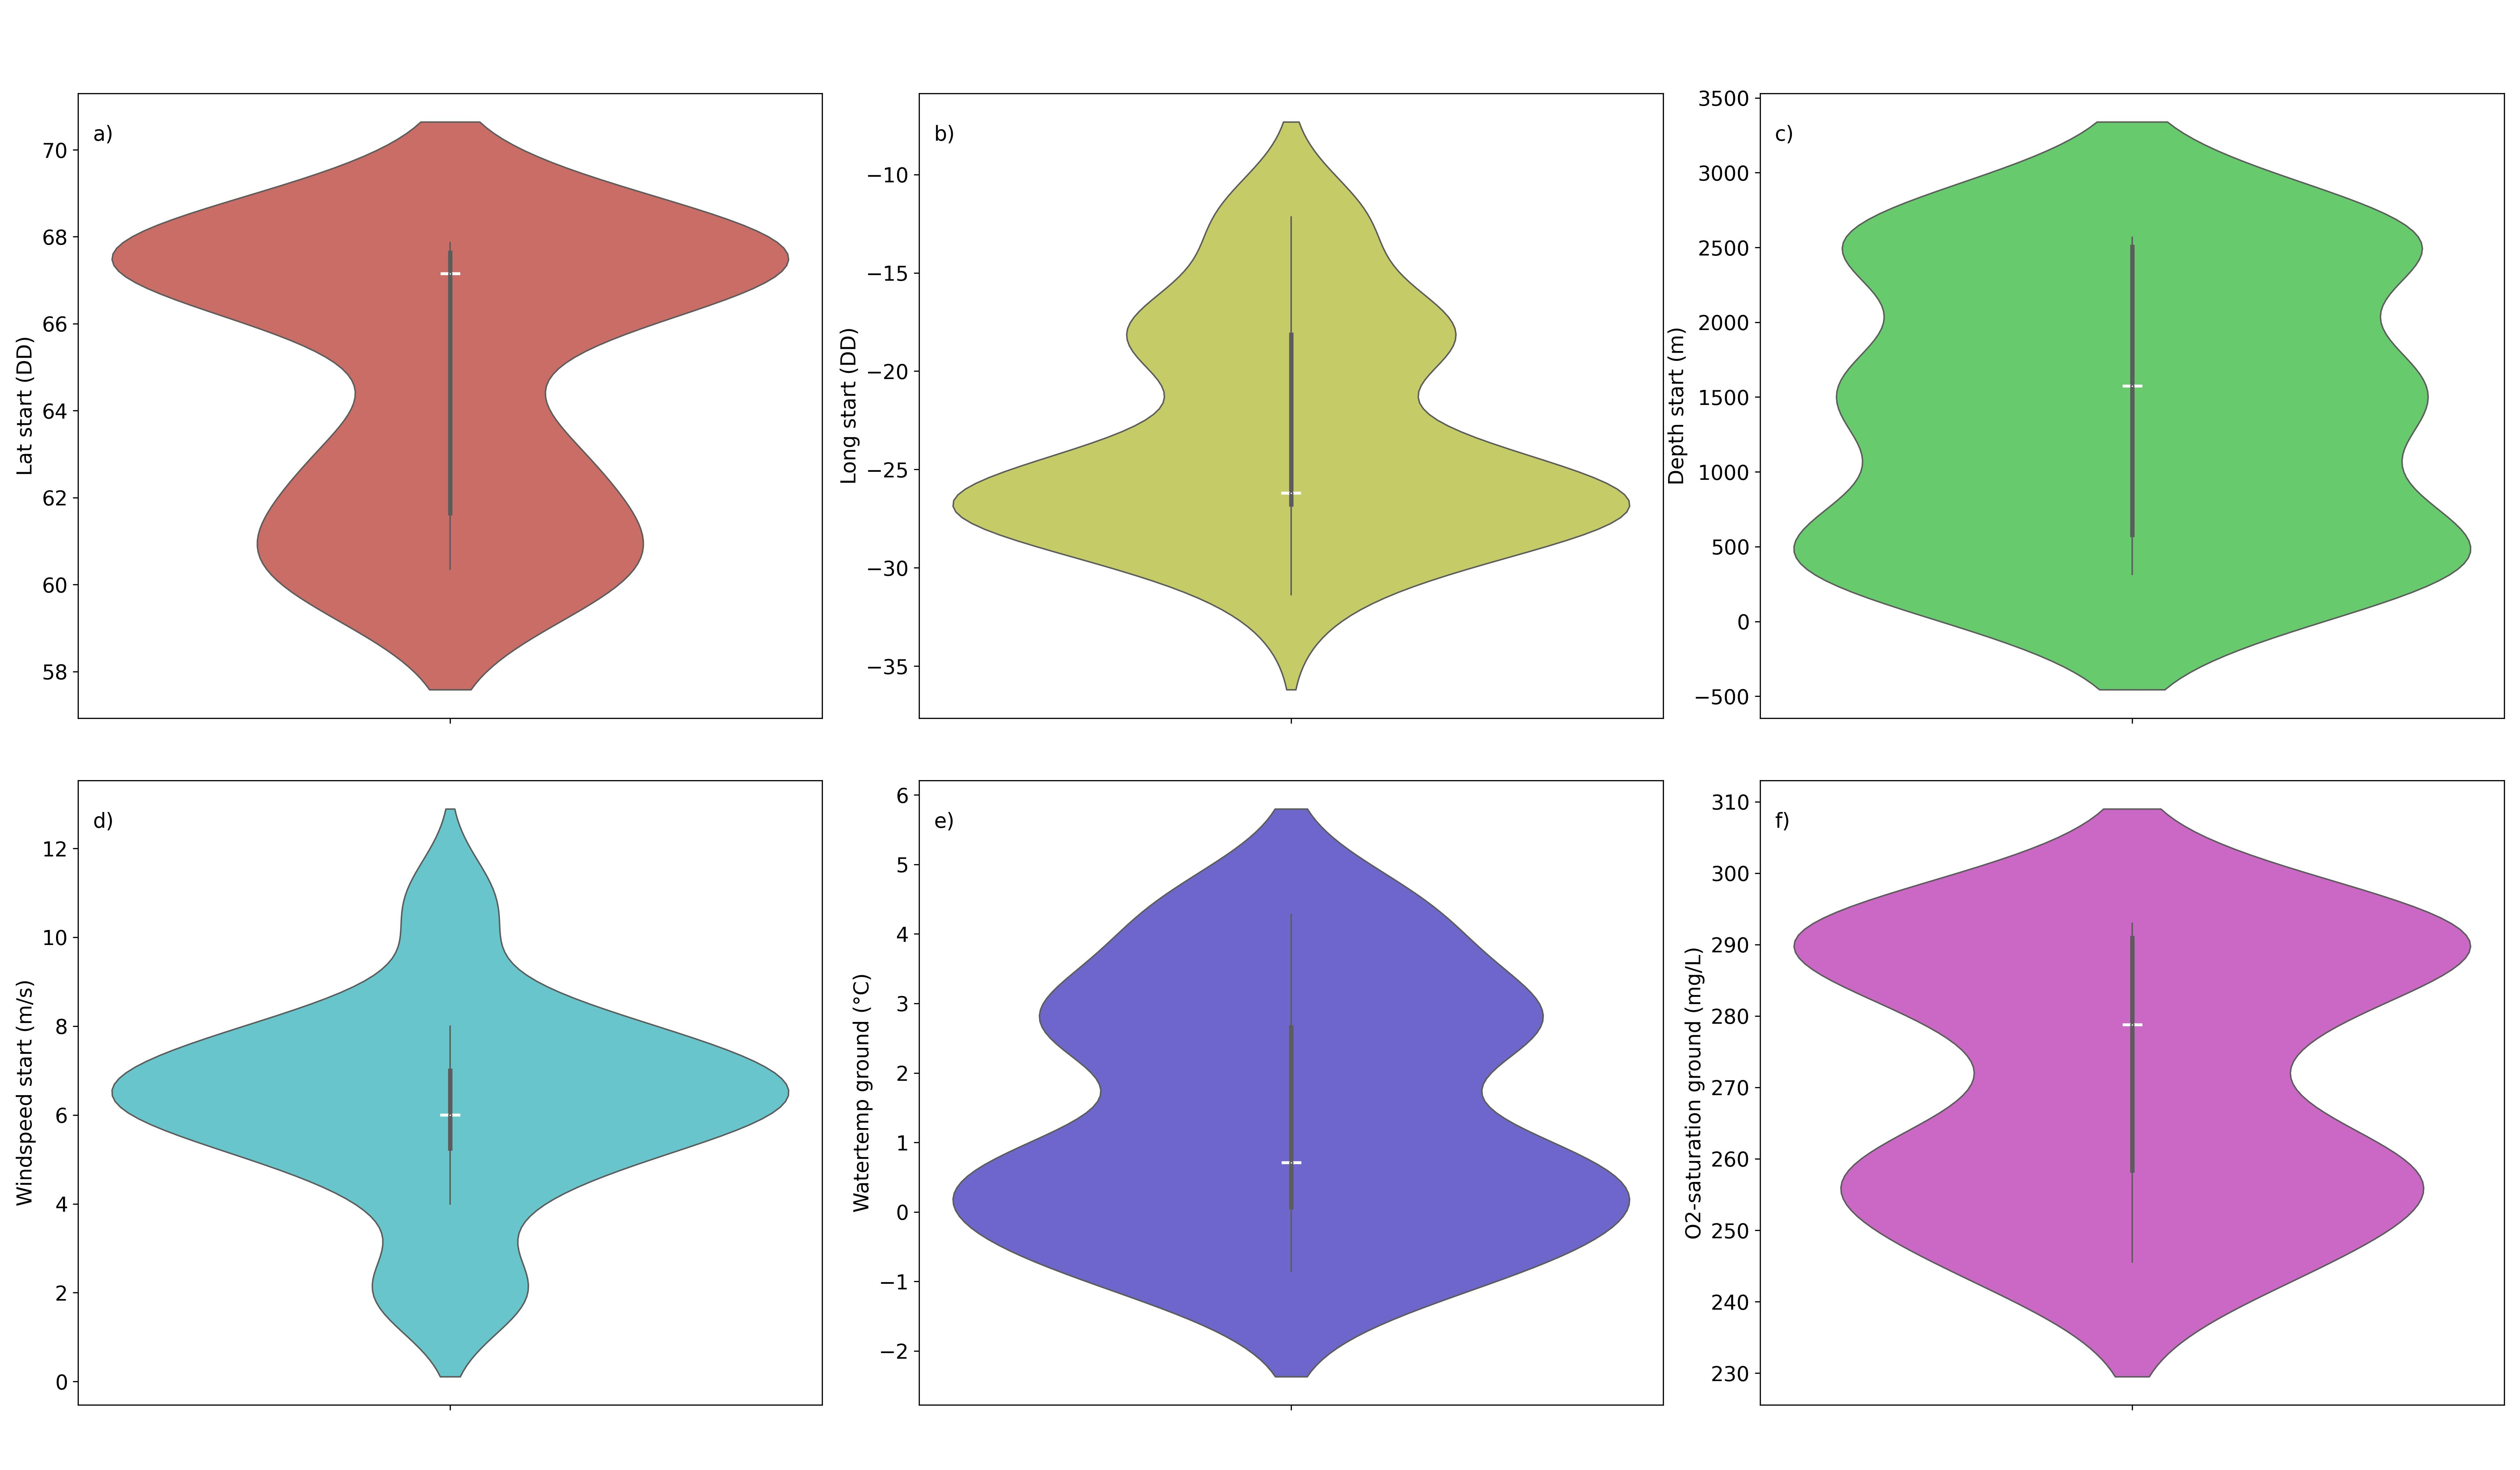
\includegraphics[width=0.7\textwidth]{figure1.jpg}
    \caption{Violin diagrams of two geographical attributes, one climatic attribute, and three environmental attributes from our sample. a) Latitude (DD) at the start of sampling (red); b) Longitude (DD) at the start of sampling (yellow); c) Depth (m) at the start of sampling (green); d) Wind speed (m/s) at start of sampling (light blue); e) Water temperature ($^\circ$C) as a function of depth at which specimens were collected (dark blue); f) O\textsubscript{2} concentration (mg/L) as a function of depth at which specimens were sampled (pink). The mean, median, standard deviation (Std Dev), 1st quartile (Q1), and 3rd quartile (Q3) of the dataset for each attribute are shown in the top right-hand corner of each graph. \label{fig:fig2}}
\end{figure}

Our results revealed variability in most cumacean habitat attributes, as shown in Figure \ref{fig:fig2}. For instance, the median latitude at the start of sampling (Figure \ref{fig:fig2}a, 67.15 DD) is higher than the mean (64.83 DD), showing an asymmetric distribution skewed towards lower values. This trend is also observed for depth (m) at the start of sampling (Figure \ref{fig:fig2}c ) and water O\textsubscript{2} concentration (mg/L) (Figure \ref{fig:fig2}f), indicating that sampling took place in regions with varied environmental contexts. The bimodal shape of the latitude distribution curve (Figure \ref{fig:fig2}a) suggests that samples came from two dominant latitudinal regions at the start of sampling. This bimodality is reflected in longitude (DD) at the beginning of sampling (Figure \ref{fig:fig2}b), as well as for temperature ($^\circ$C) (Figure \ref{fig:fig2}e) and O\textsubscript{2} concentration (mg/L) of the water (Figure \ref{fig:fig2}f), suggesting fluctuations in climatic and environmental conditions in these areas.  

The median in Figure \ref{fig:fig2}b (-26.21 DD) is lower than the mean (-23.12 DD), indicating asymmetry on the higher sides, as does the water temperature ($^\circ$C) (see Figure \ref{fig:fig2}e). The standard deviation (5.52 DD) and quartiles Q1 (-26.77 DD) and Q3 (-18.14 DD) indicate a relatively wide range, around the mean (-23.12 DD), of the longitude distribution at the start of sampling (-31.356 - -12.162 DD). This suggests a strong environmental gradient, geographical distribution and sample diversity from east to west in the region studied. The standard deviation of Figure \ref{fig:fig2}c is quite high (881.16 m), indicating high variability in sample collection depths (316 – 2568 m) and giving a more global overview of benthic habitats. Unlike all the other diagrams in Figure \ref{fig:fig2}, the curve in Figure \ref{fig:fig2}c has a multimodal shape with three prominent peaks, suggesting that the samples were mainly collected and concentrated at three different depths (around 500, 1500 and 2500 m).

The mean (6.26 m/s) and median (6.00 m/s) in Figure \ref{fig:fig2}d are the only ones in Figure \ref{fig:fig2} to be similar, indicating a symmetrical distribution, with a high concentration of data around the median (6.00 m/s). This suggests stable wind conditions (m/s) at the start of sampling. The standard deviation of Figure \ref{fig:fig2}e is relatively high (1.73 $^\circ$C) compared to the mean (1.45 $^\circ$C), indicating a wide range of water temperatures where samples were taken (0.851 – 4.28 $^\circ$C). This suggests the acclimatization of cumacean to a variety of habitat temperatures. The range of O\textsubscript{2} concentration data (see Figure \ref{fig:fig2}f) shows some variability (245.53 – 292.97 mg/L) in the environmental conditions of the sampled areas, as shown by the standard deviation (18.11 mg/L) and quartiles Q1 (258.39 mg/L) and Q3 (290.90 mg/L). These latest results reflect a diversity of O\textsubscript{2} requirements, with organisms adapted to low O\textsubscript{2} conditions and potentially influenced by the heterogeneity of biogeochemical cycles, such as photosynthesis, respiration, and organic decomposition, which have an impact on depth-dependent dissolved  O\textsubscript{2} levels.

\begin{figure}[htbp]
    \centering
    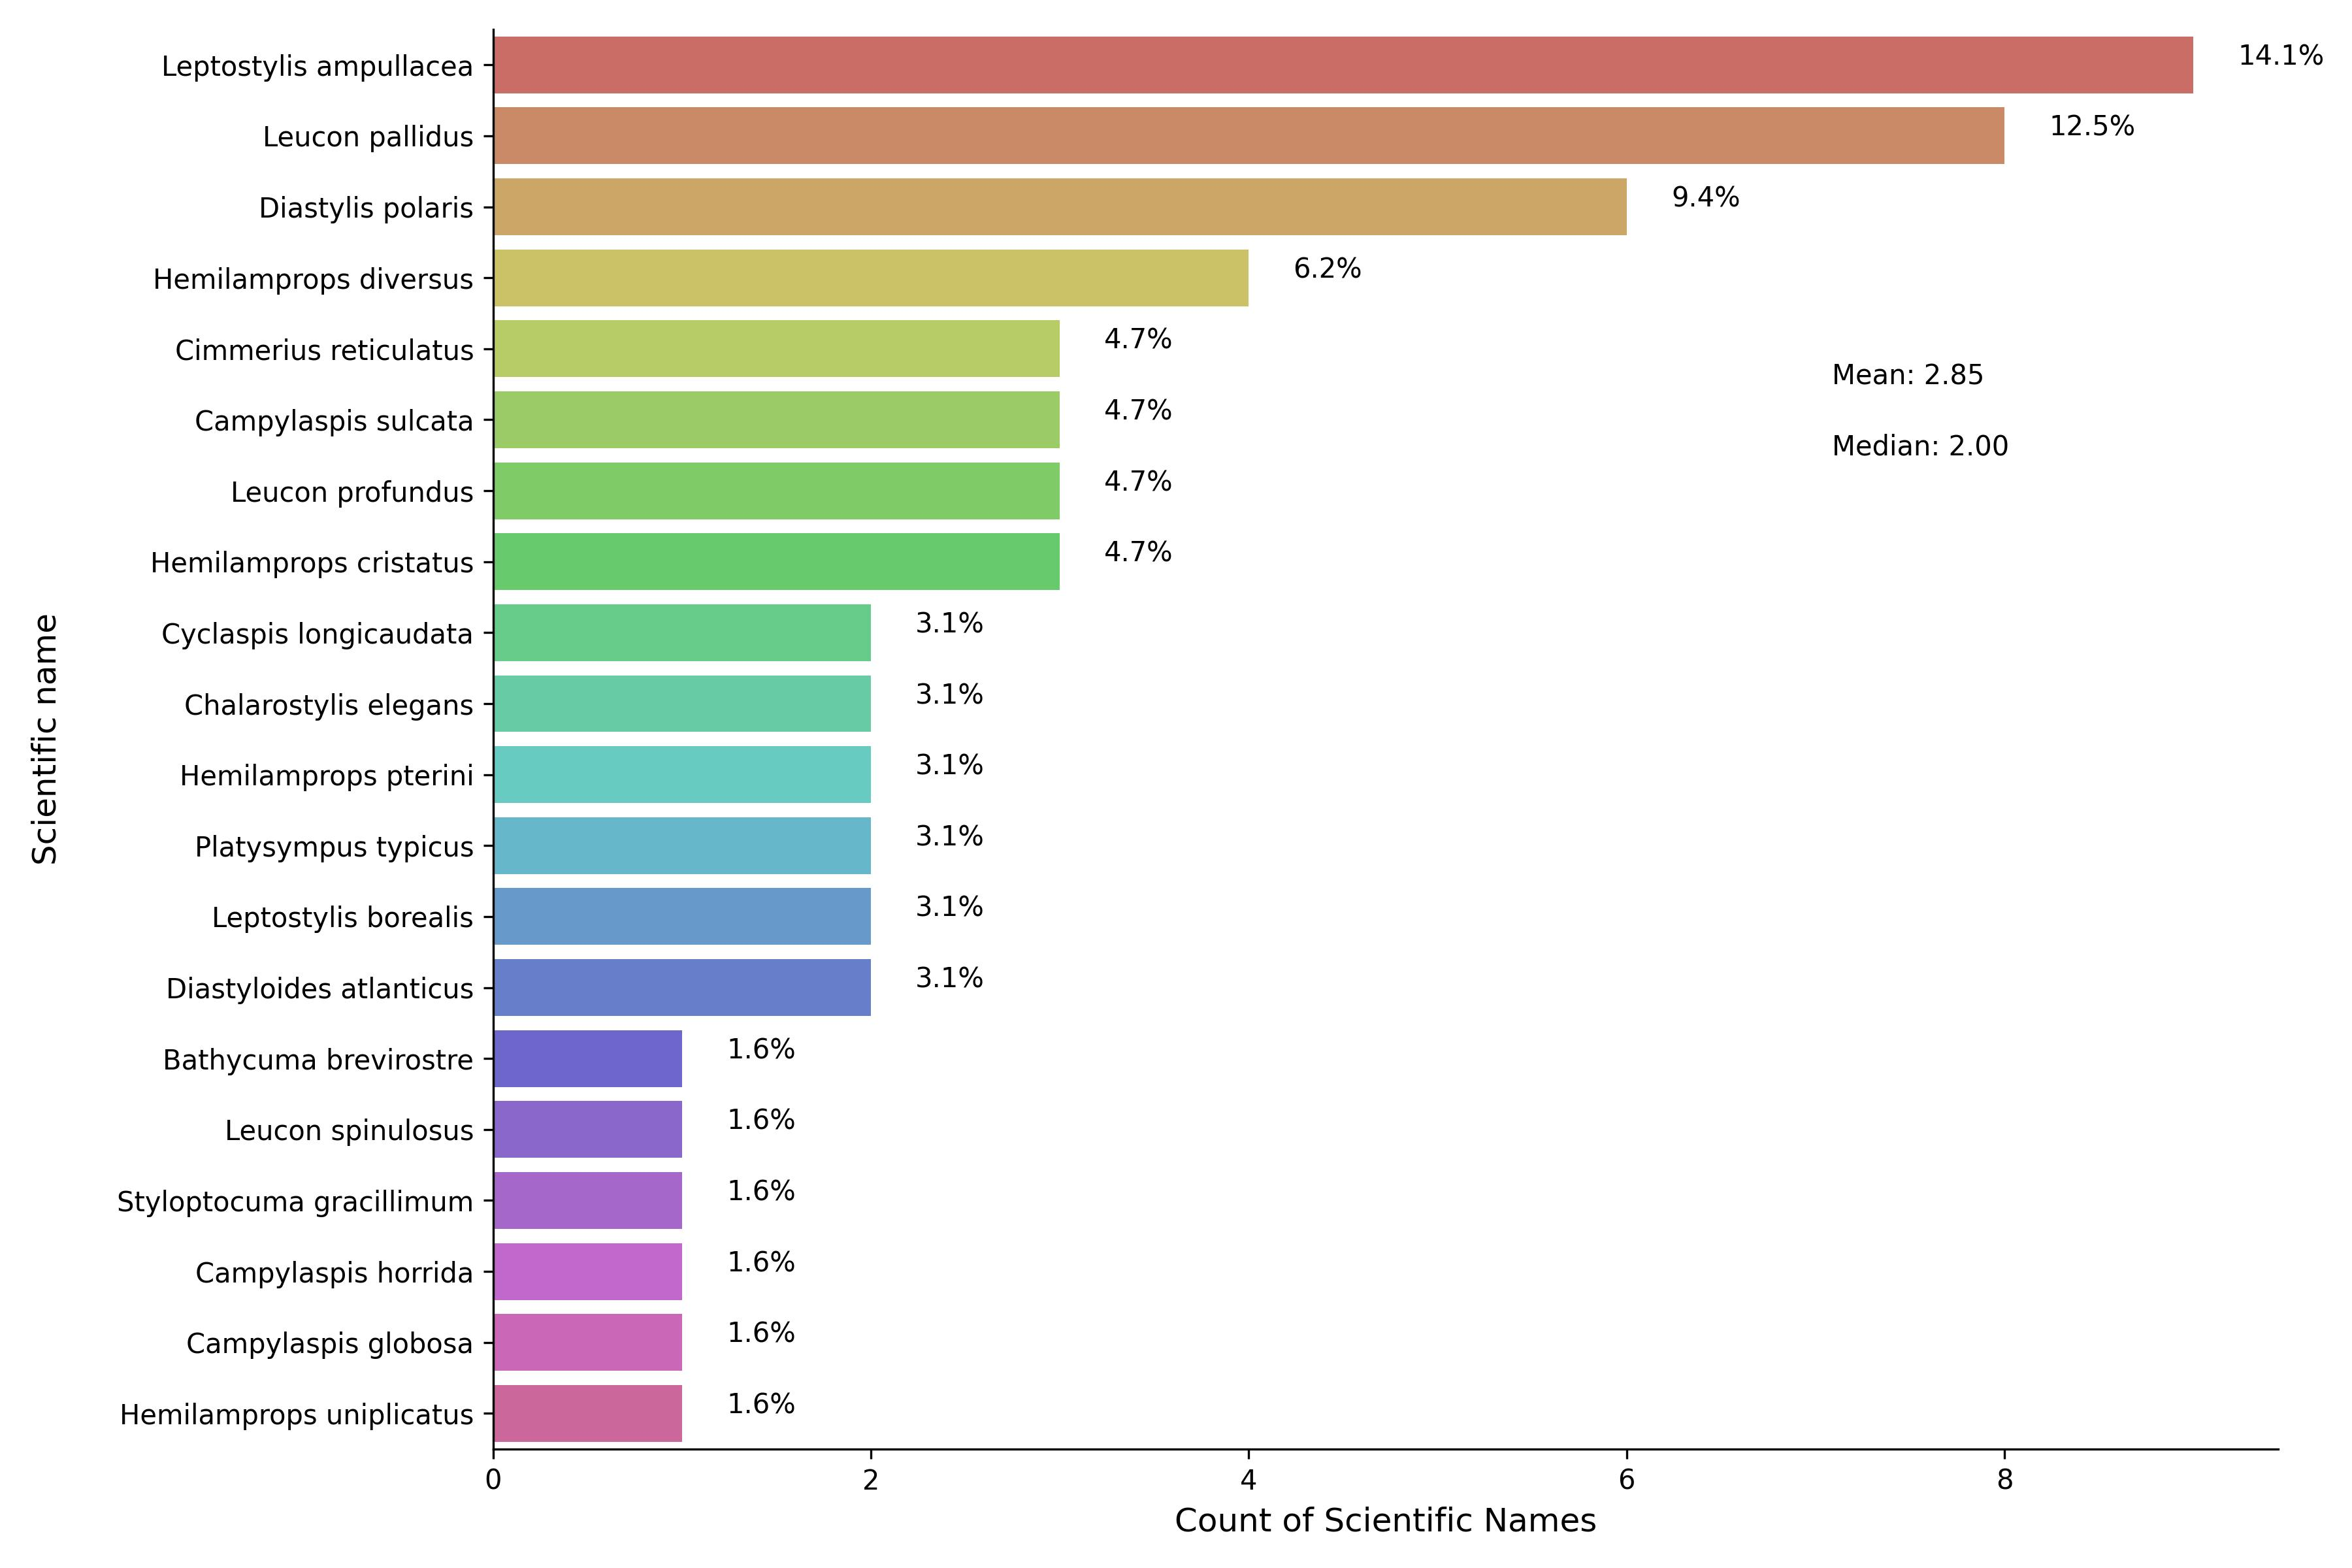
\includegraphics[width=0.7\textwidth]{figure2.jpg}
    \caption{Frequency distribution of cumacean species in our sample. The bars represent the number of individuals for each species. The percentages (\%) displayed above the bars indicate the relative abundance of each species in the total sample. The mean and median values of the frequency distribution are shown in the top right-hand corner of the histogram. \label{fig:fig3}}
\end{figure}

The distribution and diversity of the various cumacean species found in our sample are shown in Figure \ref{fig:fig3}. It shows that the most represented species are (\emph{Leptostylis ampullacea} (14.1\%) and \emph{Leucon pallidus} (12.5\%). In contrast, species like \emph{Bathycuma brevirostre} and \emph{Styloptocuma gracillimum} are less represented (1.6\%), implying that some species may have restricted ecological niches or face ecological forces that limit their distribution. The dominance of certain species (such as \emph{Leptostylis ampullacea} and \emph{Leucon pallidus}) suggests that they may have adaptive traits that enable them to make the most of the accessible resources, resist interspecific competition, or survive in fluctuating environmental conditions, which is in line with our study's aim of relating genetic adaptation to habitat attributes. 

\begin{figure}[htbp]
    \centering
    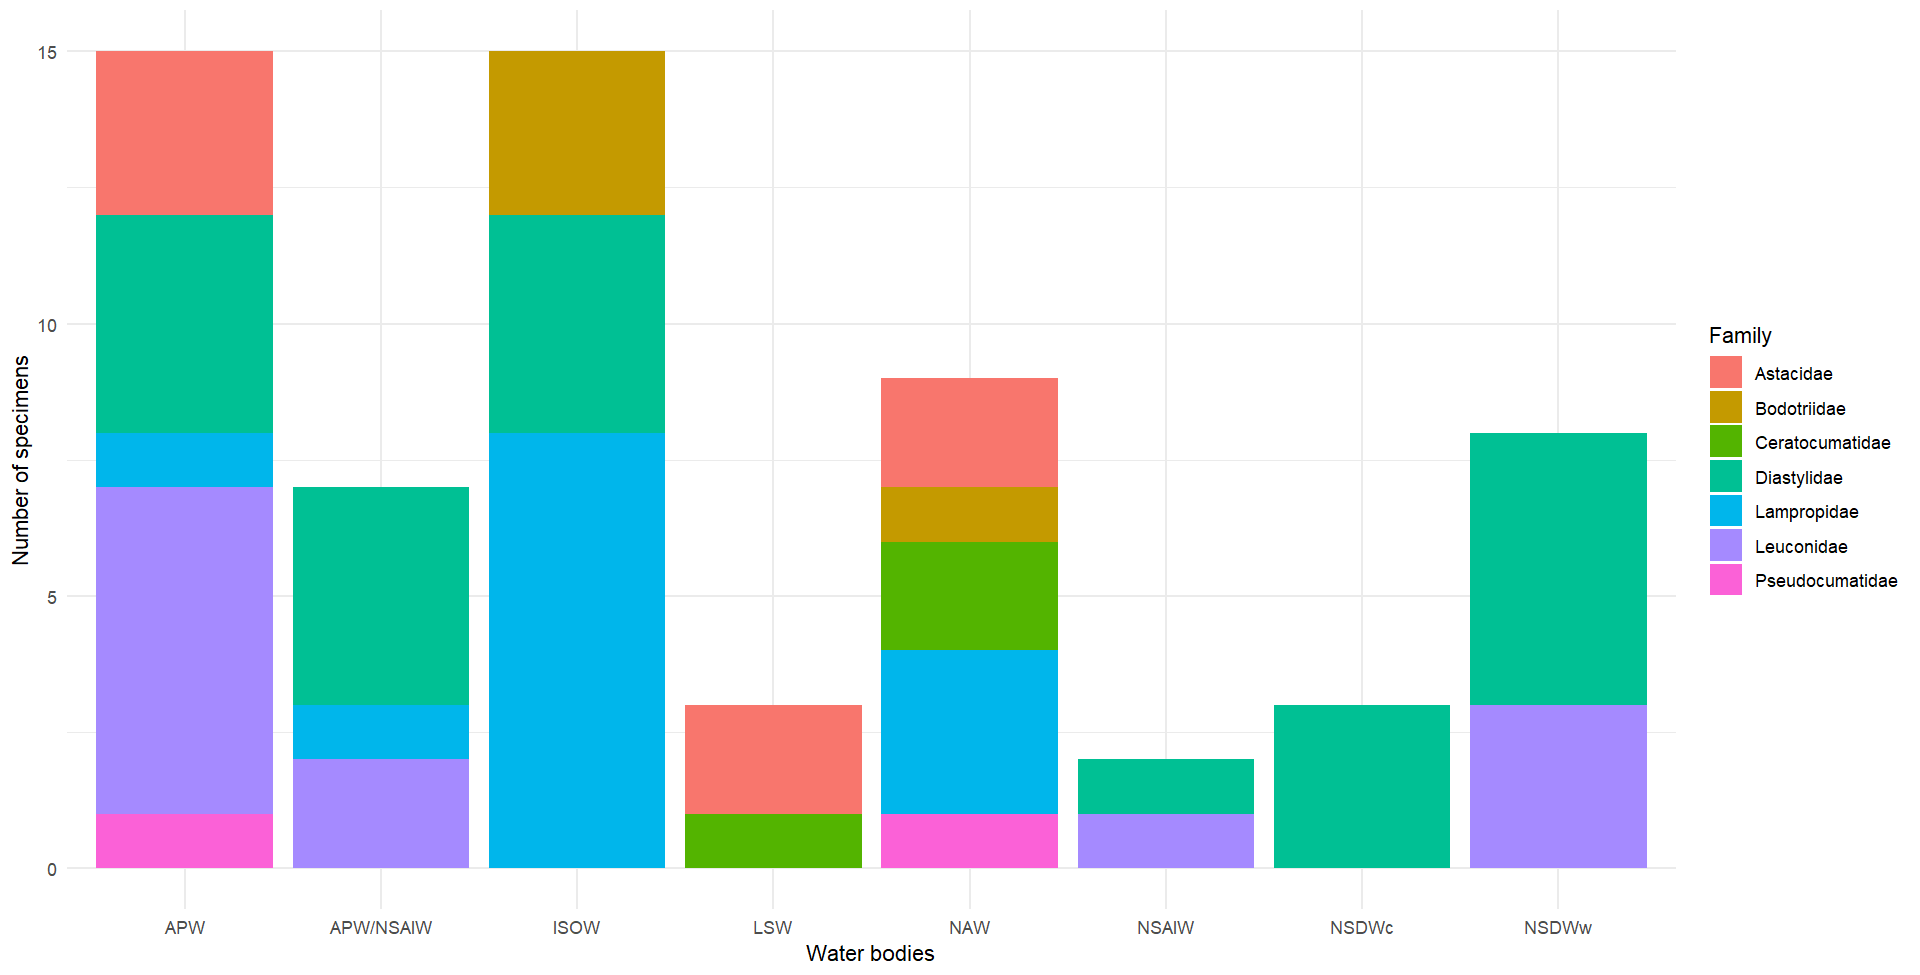
\includegraphics[width=0.7\textwidth]{figure3.png}
    \caption{Distribution of cumacean families by water mass. This histogram represents the frequency of occurrence of the different cumacean families in our samples, classified according to the water mass in which they were collected. Eight water mass categories are represented: Arctic Polar Water (APW), Arctic Polar Water/North Sub-Arctic Intermediate Water (APW/NSAIW), Iceland Scotland Overflow Water (ISOW), Labrador Sea Water (LSW), North Atlantic Water (NAW), North Sub-Arctic Intermediate Water (NSAIW), cold North Sub-Atlantic Deep Water (NSDWc), and warm North Sub-Atlantic Deep Water (NSDWw). Seven families are represented: Astacidae (red), Bodotriidae (brown), Ceratocumatidae (green), Diastylidae (turquoise), Lampropidae (blue), Leuconidae (purple), and Pseudocumatidae (pink). \label{fig:fig4}}
\end{figure}

The following figure supports the objective of our study by showing the distribution of the various cumacean families in the different water bodies (Figure \ref{fig:fig4}). The Diastylidae family, for example, is the most common in all water bodies (turquoise color in Figure \ref{fig:fig4}), testifying to its resilience and ecological adaptability to a wide variety of environmental conditions, reminiscent of the dominance of \emph{Leptostylis ampullacea} (Figure \ref{fig:fig3}, 14.1\%) which belongs to the Diastylidae family. 

\begin{figure}[]
    \centering
    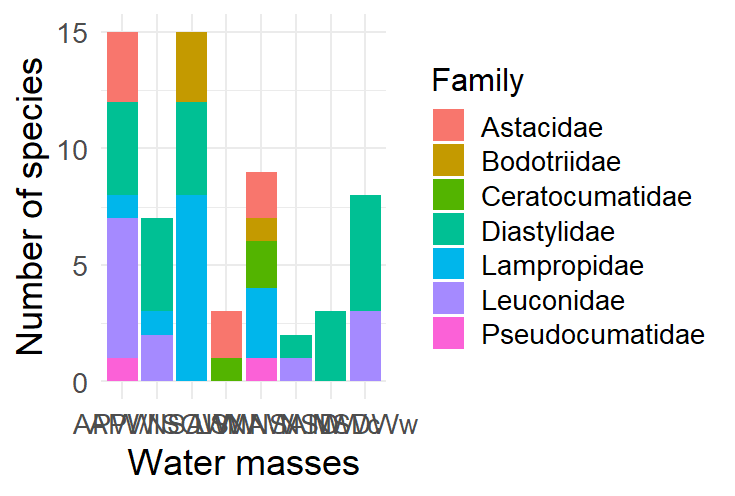
\includegraphics[width=0.7\textwidth]{figure4.png}
    \caption{Distribution of cumacean families by habitat. This histogram represents the frequency of occurrence of the different cumacean families in our samples, classified according to the habitat in which they were collected. Three habitat categories are represented: Deep sea, Shelf, and Slope. Seven families are represented: Astacidae (red), Bodotriidae (brown), Ceratocumatidae (green), Diastylidae (turquoise), Lampropidae (blue), Leuconidae (purple), and Pseudocumatidae (pink). \label{fig:fig5}}
\end{figure}

The distribution of samples of the different cumacean families according to the type of habitat where they were collected during sampling is shown in Figure \ref{fig:fig5}. The deep-sea habitats show the greatest diversity of families, mainly Diastylidae and Lampropidae, suggesting they are well acclimatized to deep-sea conditions. In contrast, the slope has the lowest diversity, with Diastylidae again the most dominant, implying that some cumacean species have fewer ecological niches or are less adapted to this habitat. Although less diverse than the deep sea, the shelf is dominated by Leuconidae, indicating that this family may be specifically well-acclimated to shelf environments. These patterns reinforce the hypothesis that certain cumacean families, such as the Diastylidae, Lampropidae, and Leuconidae, have developed distinct adaptations (physiological, behavioral or morphological) to remain in particular ecological niches, reflecting the impact of habitat conditions on the genetic distribution of cumacean.

\begin{figure}[]
    \centering
    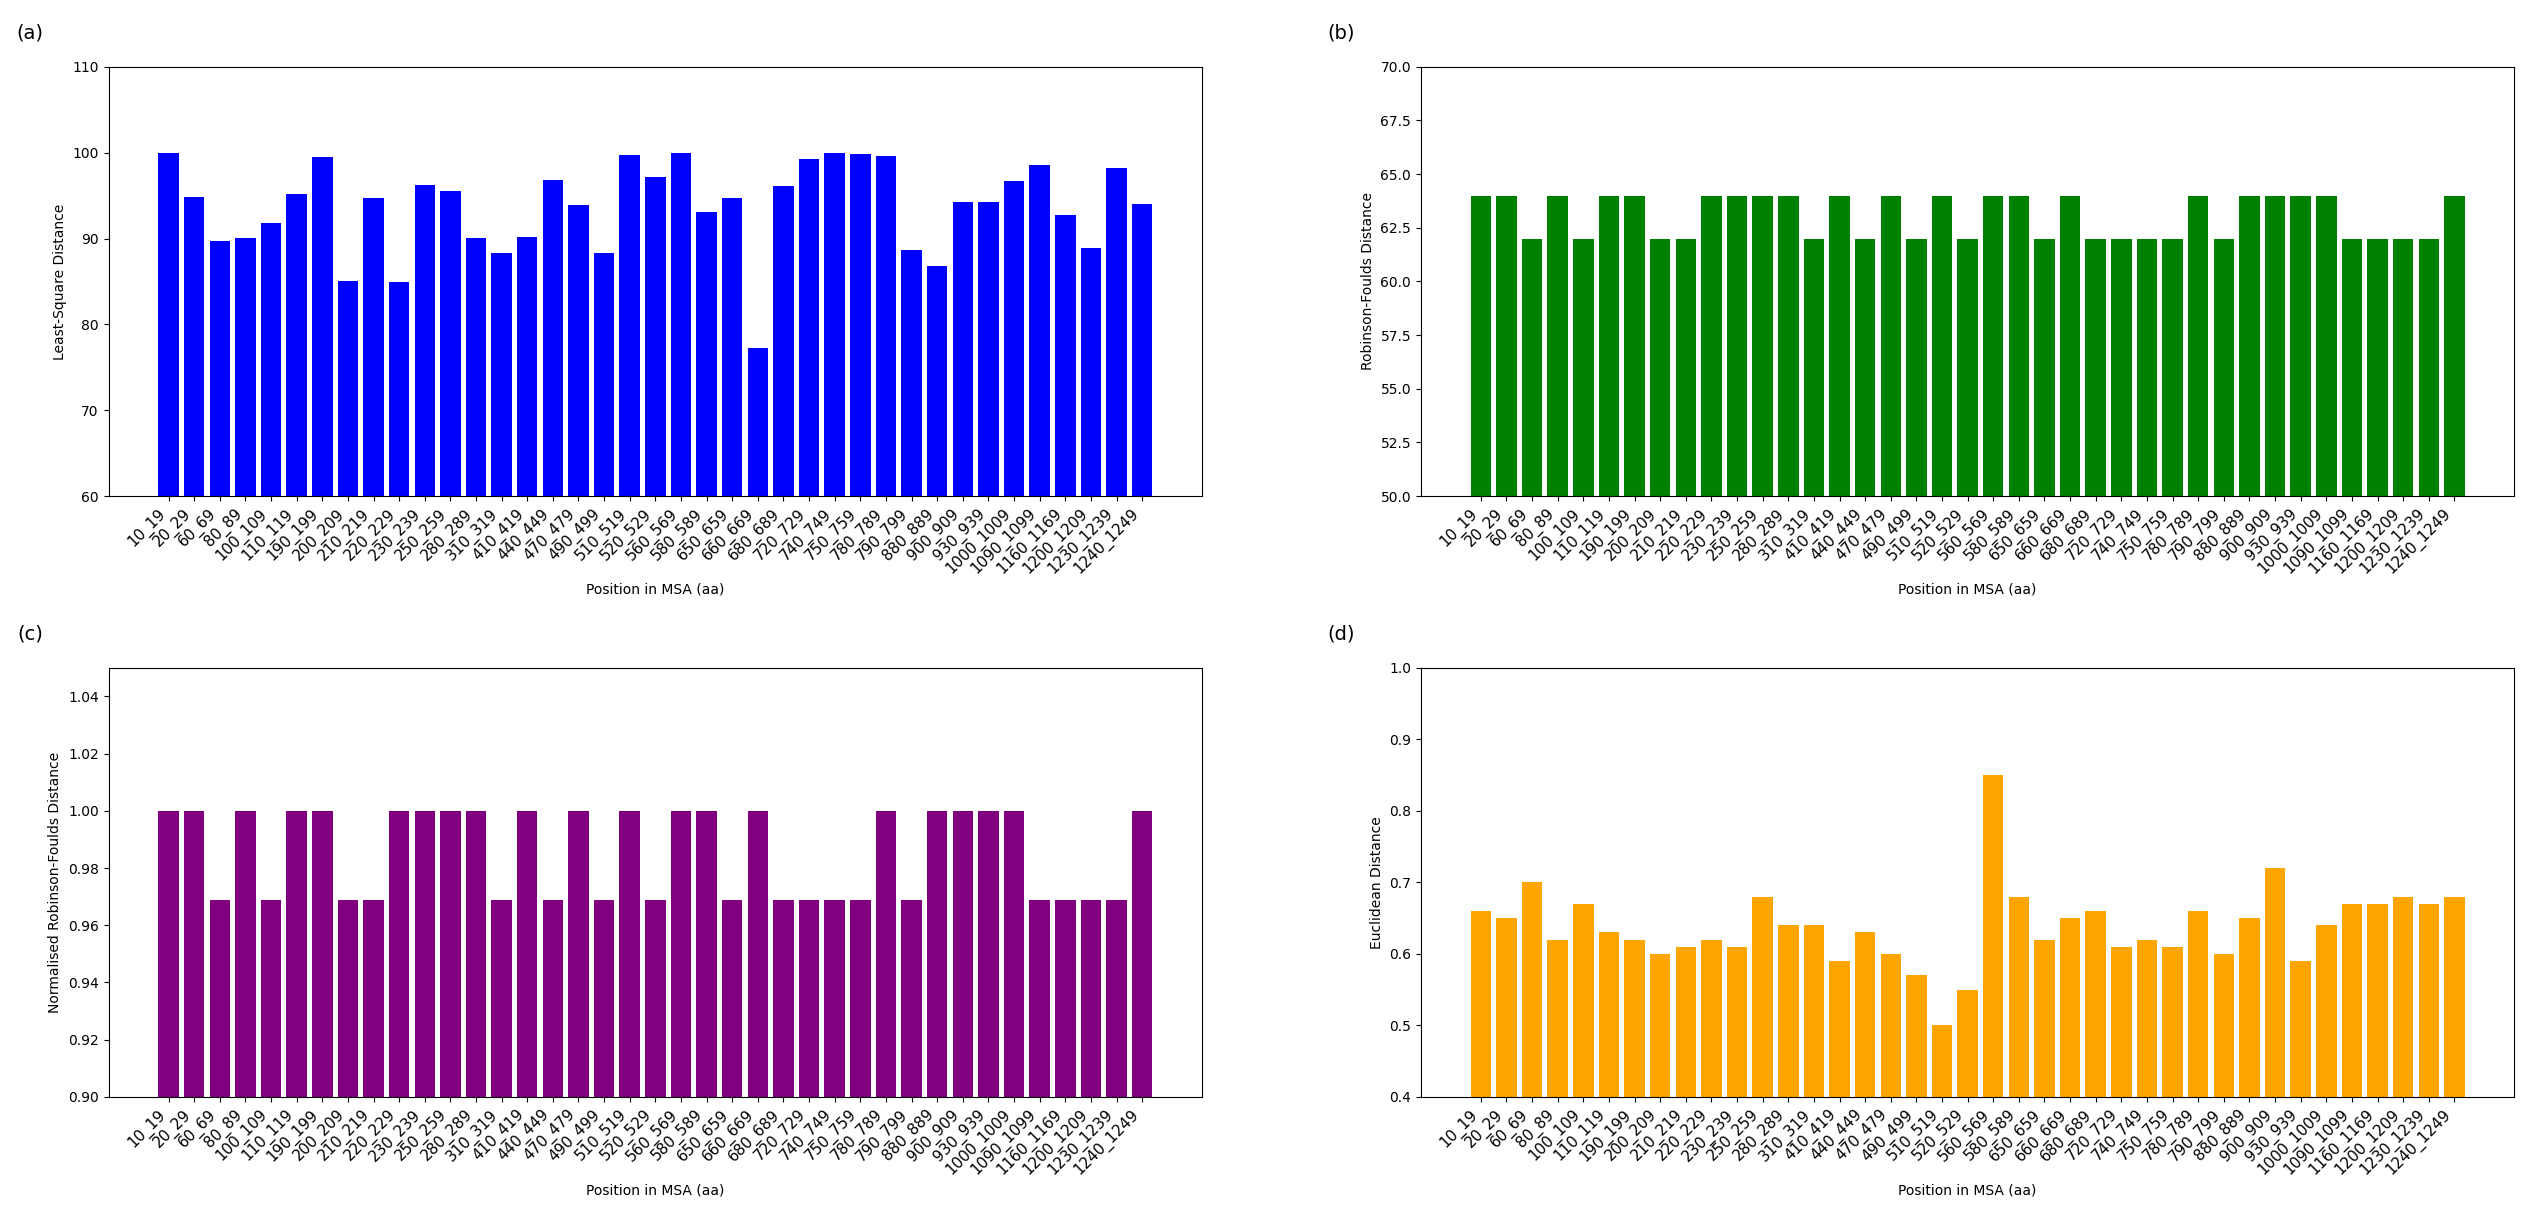
\includegraphics[width=0.7\textwidth]{figure5.png}
     \caption{Analysis of fluctuations in four distance metrics using multiple sequence alignment (MSA): a) Least-Squares Distance (LSD), b) Robinson-Foulds Distance (RFD), c) normalized Robinson-Foulds Distance (nRFD), and d) Euclidean Distance (ED). These distance variations are studied to establish their correlation with the variation in wind speed (m/s) at the start of sampling. \label{fig:fig6}}
\end{figure}

\begin{figure}[]
    \centering
    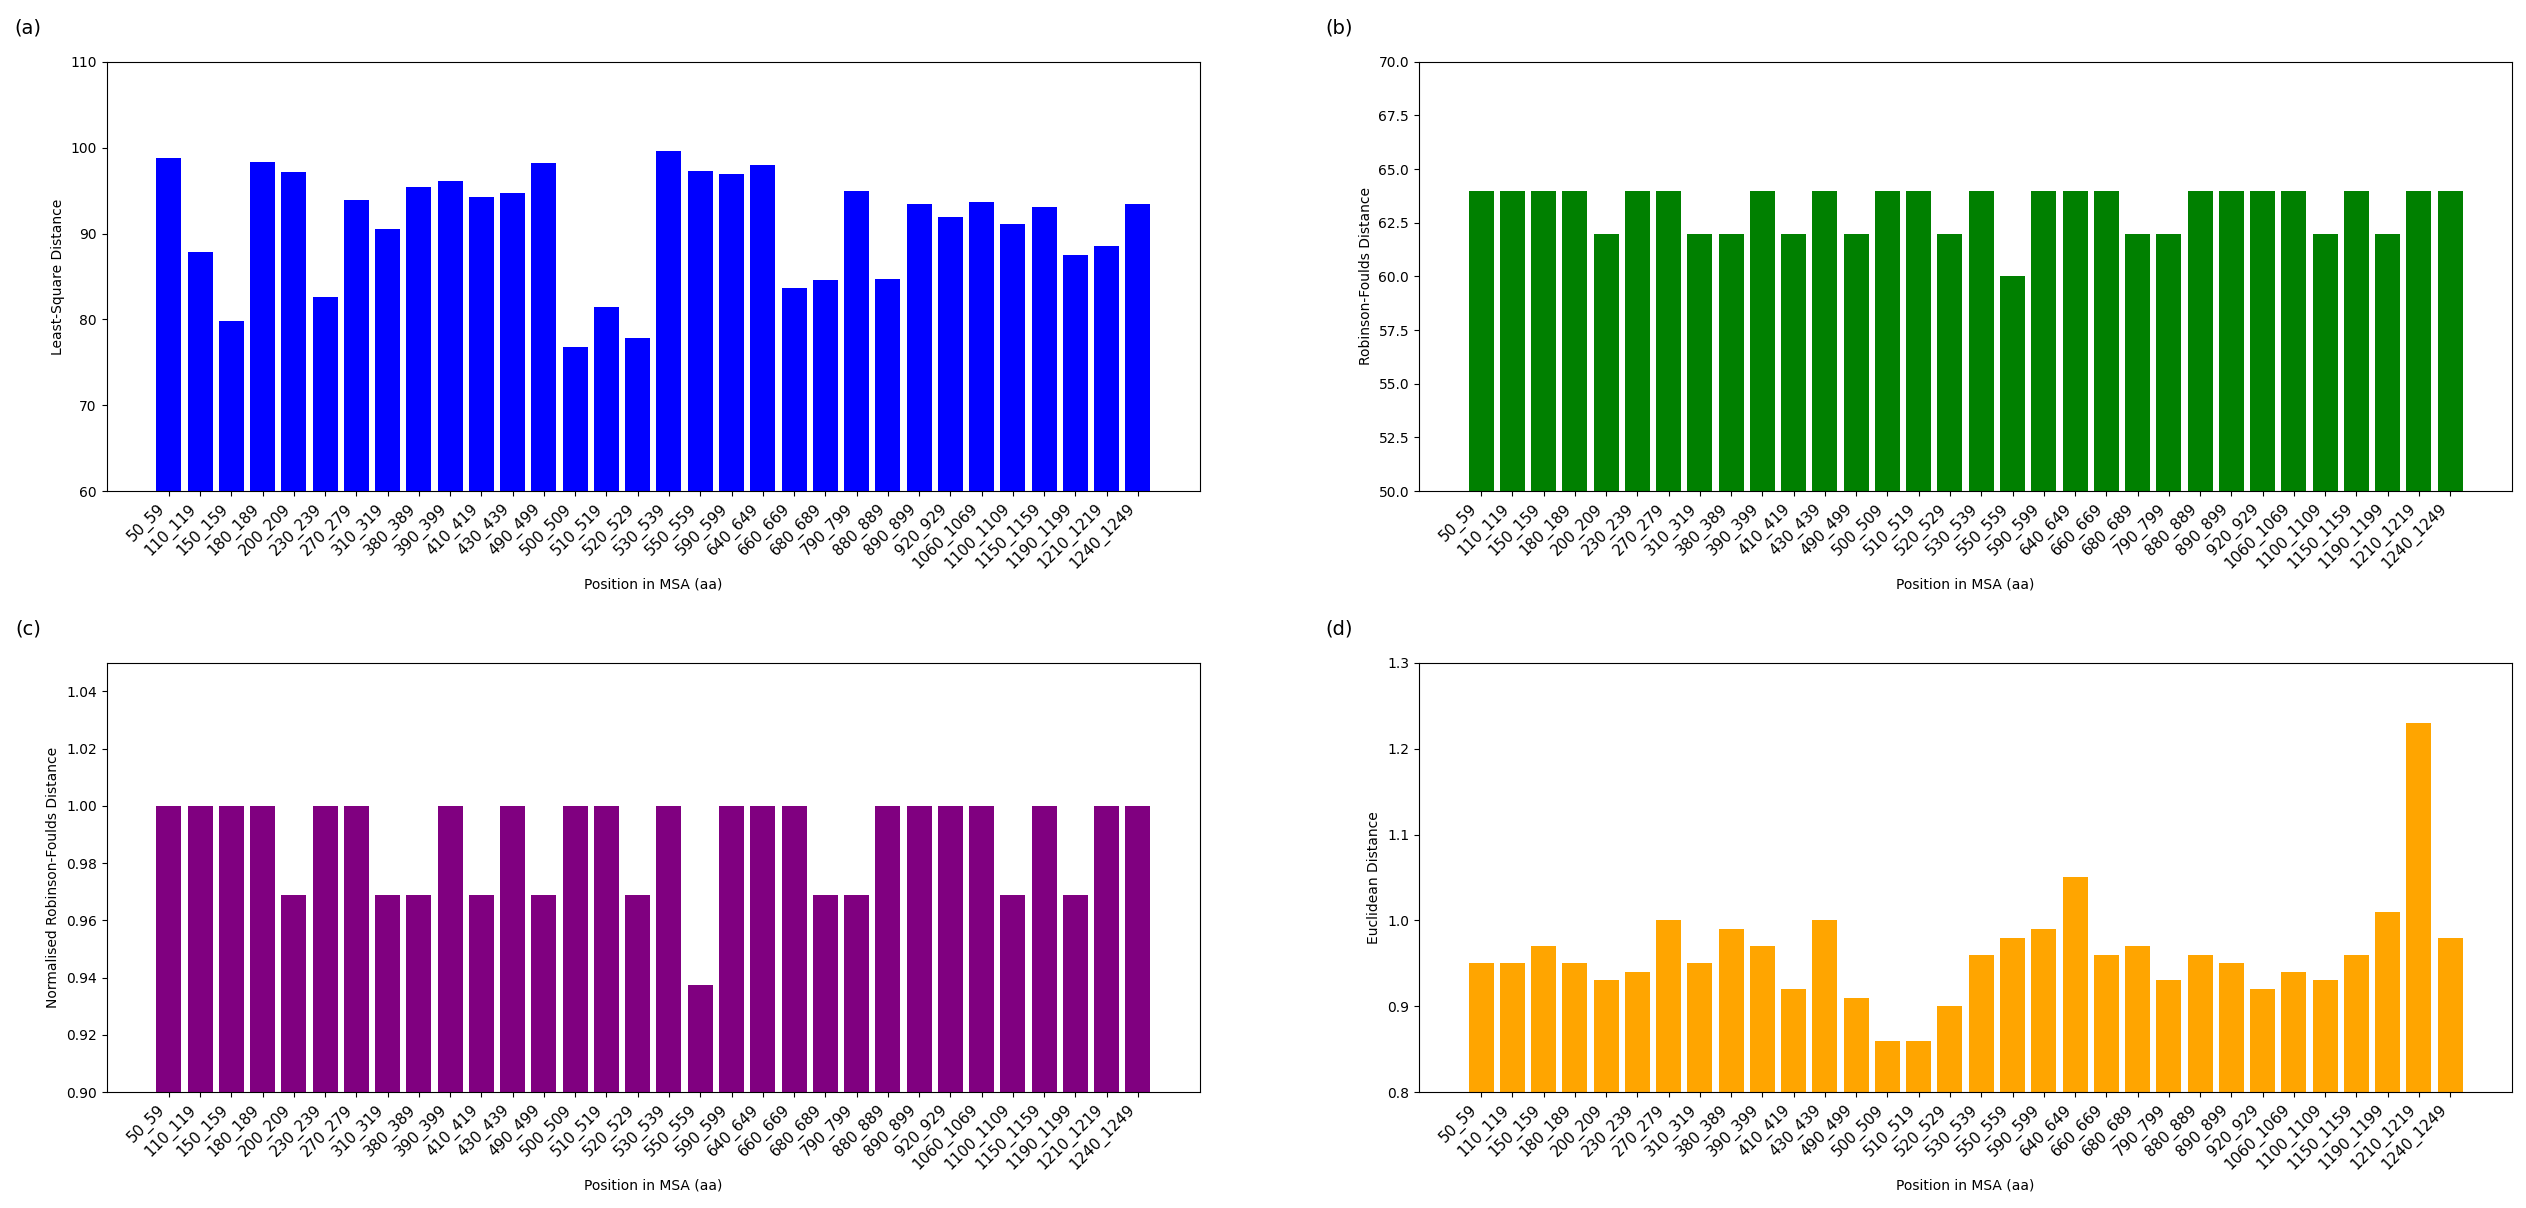
\includegraphics[width=0.7\textwidth]{figure6.png}
    \caption{Analysis of fluctuations in four distance metrics using multiple sequence alignment (MSA): a) Least-Squares Distance (LSD), b) Robinson-Foulds Distance (RFD), c) normalized Robinson-Foulds Distance (RFD), and d) Euclidean Distance (ED). These distance variations are studied to establish their correlation with variation of O\textsubscript{2} concentration (mg/L) at the sampling sites. \label{fig:fig7}}
\end{figure}

The correlation between the genetic sequences and two attributes, one climatic (wind speed (m/s) at the start of sampling) and the other environmental (O\textsubscript{2} concentration (mg/L)) is presented in Figure \ref{fig:fig6} and Figure \ref{fig:fig7}. All the attributes given in the first step of the \textit{aPhyloGeo} software section were analyzed (see \autoref{aPhyloGeo-software}) and are available in the img and script python file on \href{https://github.com/tahiri-lab/Cumacea_aPhyloGeo}{GitHub}. However, only these two parameters showed the most interesting mutation rate. Using four metrics (LSD, RFD, nRFD, and ED), we noticed that the ED is particularly sensitive to our data, manifesting considerable sequence variation at positions 520-529 amino acids (aa) (ED: 0.8 < x < 0.9; Figure \ref{fig:fig6}d) and 1190-1199 aa (ED: 1.2 < x < 1.3; Figure \ref{fig:fig7}d). This implies that these genetic sites are subject to selection pressures or evolutionary changes, due to environmental (O\textsubscript{2} concentration) and climatic conditions (wind speed). This is in line with the aim of our study, which is to identify the cumacean genetic region with the highest mutation rate linked to an attribute of its habitat.

These results provide important insight into the genetic adaptation of cumaceans to their environment. These results need to be analyzed in greater depth to certify their involvement, especially in contrast with \citep{uhlir_adding_2021}, which investigated similar topics of environmental and climatic effects on cumacean distribution and genetics.

\section{Conclusion}\label{conclusion}
This study examines the effects of climatic, geographic, and environmental characteristics on the genetics of cumaceans in the waters surrounding Iceland. Our main objective is to determine whether there is a  correlation between precise genetic information of the 16S rRNA mitochondrial gene region (i.e., window) of cumacean species and their habitat attributes. In particular, we aim to identify the attribute most correlated with a specific genetic sequence and the potentially associated protein.

We meticulously curated relevant attributes from the IceAGE project data, the bold systems database, and the \citep{uhlir_adding_2021} study. Some attributes have been excluded for lack of relevance, low variance (e.g., salinity, $S^2 = 0.02146629$), abundant missing data (> 95\%), or high inter-correlation (threshold > 0.9) to guarantee the robustness of our analysis. Utilizing this refined dataset, we integrated phylogeographic studies using \textit{aPhyloGeo} software (see \autoref{lst:main}), allowing a comprehensive analysis of potential correlations between the genetics of cumacean species and their living environment. Notably, DNA sequence analyses have identified specific genetic windows with high mutation rates in response to climatic and environmental attributes such as wind speed (m/s) at the start of sampling (MSA: 520-529 aa; ED: 0.8 < x < 0.9; Figure \ref{fig:fig6}d) and O\textsubscript{2} concentration in water (mg/L) (MSA: 1190-1199 aa; ED: 1.2 < x < 1.3; Figure \ref{fig:fig7}d). These results imply variable genetic sites that could contribute to the evolutionary acclimatization of cumaceans to their fluctuating environments.

The novelty in our research lies in the exhaustive correlation between habitat attributes and genetic mutability, particularly in identifying genetic windows associated with habitat fluctuations, which has not been widely investigated in previous studies \citep{manel2003landscape, vrijenhoek2009cryptic}. In this case, our integrated method identifies specific genetic regions sensitive to environmental and climatic variations. Thus, by seeking to determine which of these two attributes is most closely correlated with their genetic sequence, the potential evidence of proteins related to one of these variable DNA sequences will enable us to depict the functional effects of this genetic adaptation.

Interpreting how marine invertebrates genetically adapt to variations in their habitat can help us better predict their responses to climate change and advance conservation plans to protect them. Recognition of these specific attributes that affect the genetic variability of cumaceans can contribute to the designation and supervision of marine protected areas, assuring they include habitats crucial to the survival and acclimatization of these species. Thus, our results can inform the management of fishing and seabed mining companies by revealing ecologically vulnerable areas where these disturbances can seriously affect benthic biodiversity.

Furthermore, our results provide essential knowledge to guide future studies on the genetic adaptation of cumaceans and other invertebrates to ecological and geographic variability. On this basis, future research should focus on additional environmental and climatic attributes, such as nutrient accessibility, water pH, ocean currents, and the degree of human disturbance, to further improve the interpretation of the complex interactions between genetics and the environment. Broadening the scope of application to other marine species, not just marine invertebrates, and diverse geographical regions would allow us to generalize the results more effectively. With this in mind, longitudinal study models on these species could reflect long-term climatic and environmental fluctuations and improve our knowledge of the dynamics of genetic acclimatization.

However, it is important to acknowledge the limitations of our study. In particular, the three missing data points on O\textsubscript{2} concentration (mg/L) in the water and the relatively small sample size ($n=62$) could have an impact on the interpretations and generalization of our results. Future studies should address these limitations by increasing sample sizes and guaranteeing complete datasets to confirm and expand our results. In addition, as our research focuses only on the mitochondrial sequence of the 16S rRNA gene, utilizing more elaborate genomic methods, such as whole-genome sequencing, could help us better understand the genetic variety of marine species and their acclimatization mechanisms. Finally, multidisciplinary efforts between ecology, genetics, and oceanography would be essential to optimize knowledge sharing and its use in future research.

\section{Acknowledgments}\label{acknowledgments}
The authors thank the SciPy conference and reviewers for their valuable comments on this paper as well as Mansour Kebe for his technical support and Carolin Uhlir for her clarifications and advice on her study \citep{uhlir_adding_2021}. This work was supported by the Natural Sciences and Engineering Research Council of Canada (NSERC), the Fonds de recherche du Québec - Nature et technologies (FRQNT), the Université de Sherbrooke grant, and the Centre de recherche en écologie de l’Université de Sherbrooke (CREUS).
